Nel caso preso in esame da questo elaborato il controllo di assetto prende in
considerazione una fase scientifica, per tanto mira a mantenere dei requisiti di
precisione nell'assetto stringenti, l'assetto va mantenuto allineato con un
riferimento \emph{LORF}, il controllo è di tipo attivo, prevede come schema a
blocchi di alto livello quello mostrato in figura \ref{fig:attitude_control}
composto dai seguenti blocchi funzionali:
\begin{description}
\item[Generatore dei riferimenti:] Fornisce il quaternione di assetto di
riferimento,la velocità angolare di riferimento, e l'accelerazione angolare di
riferimento, il controllo dovrà minimizzare l'errore rispetto al riferimento
\item[Predittore dello stato (Embedded Model + Noise Estimator):] permette di
calcolare in anticipo la legge di controllo fornendo la predizione a un passo,
sulla base dei passi precedenti, dello stato. Sfrutta la misura dello startracker.
\item[Legge di controllo:] Calcola le coppie necessarie a minimizzare l'errore
rispetto al riferimento dell'assetto corrente.
\end{description}

 \begin{figure}[ht!]
\includegraphics[width=\textwidth,page=24,clip=true,trim=2.8cm 17cm 2.7cm 3.5cm]{control/attitude_control/images/attitude_control.pdf}
\caption{Schema a blocchi del controllo di assetto}
\label{fig:attitude_control}
\end{figure}